\documentclass[sigconf]{acmart}
\AtBeginDocument{%
  \providecommand\BibTeX{{%
    \normalfont B\kern-0.5em{\scshape i\kern-0.25em b}\kern-0.8em\TeX}}
    }

\setcopyright{acmcopyright}
\acmConference[CZ4045]{CZ4045 Natural Language Processing, Nanyang Technological University}{November 04, 2019}{Singapore}

\begin{document}

\title{Assignment Report}
\subtitle{NTU CZ4045 Natural Language Processing}

\author{Li Bingzi}
\authornote{Li Bingzi contributes to the writing style analysis and sentence segmentation}
\affiliation{%
  \institution{U1722793H}
}
\email{LI0001ZI@e.ntu.edu.sg}

\author{Li Guanlong}
\authornote{Li Guanlong contributes to the tokenization and stemming analysis}
\affiliation{%
  \institution{U1722033H}
}
\email{GLI009@e.ntu.edu.sg}

\author{Wu Ziang}
\authornote{Wu Ziang contributes to the POS tagging and application of sentiment analysis}
\affiliation{%
  \institution{U17224323H}
}
\email{ZWU018@e.ntu.edu.sg}

\author{Yong Hao}
\authornote{Yong Hao contributes to the most frequent adjective for each rating
and pplication
}
\affiliation{%
  \institution{U1722282A}
}
\email{YO0001AO@e.ntu.edu.sg}

\author{Zhang Yuehan}
\authornote{Zhang Yuehan contributes to the None-Adjective Summarizer}
\affiliation{%
  \institution{U1722863L}
}
\email{YZHANG145@e.ntu.edu.s}


\begin{abstract}
This is the report for CZ4045 Natural Language Processing Assignment. The assignment requires to perform exercises of several Natural Language Processing techniques and develop applications based on Natural Language Processing concepts using restaurant reviews. This report composes of three sections: Data Analysis, which includes Writing Style, Sentence Segmentation, Tokenization, Stemming, POS Tagging, and Most Frequent Adjectives; Noun-Adjective Pair Summarizer; and Application of Sentiment Analysis.
\end{abstract}

\begin{CCSXML}
<ccs2012>
<concept>
<concept_id>10010147.10010178.10010179</concept_id>
<concept_desc>Computing methodologies~Natural language processing</concept_desc>
<concept_significance>500</concept_significance>
</concept>
</ccs2012>
\end{CCSXML}

\ccsdesc[500]{Computing methodologies~Natural language processing}

\keywords{Natural Language Processing, Writing Style, Sentence Segmentation, Tokenization, Stemming, POS Tagging, Summarizer, Sentiment Analysis}

\maketitle

\section{Data Analysis}

\subsection{Writing Style}

The writing style observed in restaurant reviews, the informal or causal writing style, are compared with new paper articles, the formal writing style. 

\subsubsection{Reviews} Following are some example reviews extracted from the data. Note that reviews are in a relatively causal writing style, where some proper nouns are not capitalized, e.g. "boba", several grammar errors are found, e.g. sentence "will smell like BBQ grill after" has not subject, numbers of informal words are used, e.g. ahem ahem, and some recombination of punctuations are used to express feelings, e.g. :)

\begin{itemize}
\item{Example 1}:"By far the most affordable sushi place on the west side :) I love their Hawaii Roll!! The slivers of almond get me every time!! I also love their bento special. If you're not particularly hungry, don't get it! It's a lot of food.  You can get a lot of food for under \$10.  Definitely a place to try :) ahem ahem walk over to the donut shop next door and have a boba for dessert. Just sayin!!"
\item{Example 2}:"Good Korean grill near Eaton Centre. The marinate is good. We got beef, ox liver, salmon, fish fillet, chicken, pork, pork belly. The fish fillet was bland and liver was meh. Salmon and chicken was really flavourable. Such a fun place to eat at for a date or group of friends. Even alone. No judgments here. The staff is attentive, nice and considerate. Bigger groups will most likely be seated on the second floor which is way bigger.Caution: will smell like BBQ grill after."
\end{itemize}

\subsubsection{Newspaper Articles}
One example of newspaper articles, where formal writing style is applied, i.e. all proper nouns capitalized, mostly grammatically correct, and appropriate choice of word.

\begin{itemize}
\item{The Straits Times}:"Typhoon Hagibis, which means "speed" in the Philippine language Tagalog, is due to make landfall on Japan's main island of Honshu late on Saturday, a month after one of the strongest typhoons to hit the country in recent years destroyed or damaged 30,000 houses and caused extensive power outages"
\end{itemize}

\subsection{Sentence Segmentation}
The sentence segmentation is performed on the restaurant reviews and the distributions of the number of sentences given by segmentation with respect to rating stars are shown in plots. In each plot, the x-axis is the length of a review in number of sentences, and the y-axis is the number of reviews of such length. Figure \ref{fig:seg_1star} shows the distribution of 1 star, and Figure \ref{fig:seg_2star}, \ref{fig:seg_3star}, \ref{fig:seg_4star}, and \ref{fig:seg_5star} show that of 2, 3, 4 and 5 stars respectively.

\begin{figure}[ht]
  \centering
  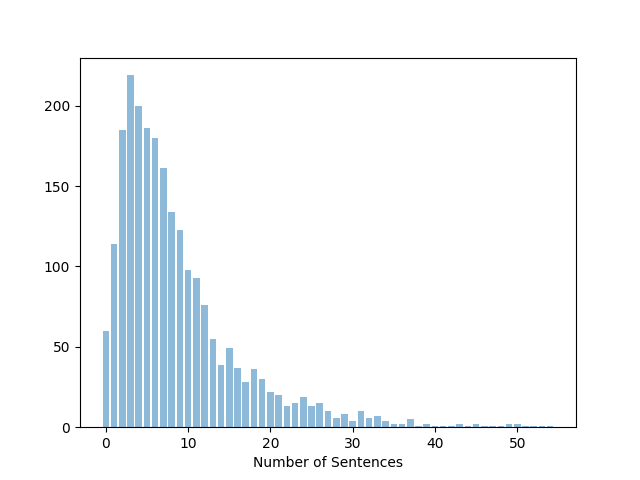
\includegraphics[width=\linewidth]{segmentation_1star.png}
  \caption{Sentence segmentation of reviews with 1 star}
  \label{fig:seg_1star}
\end{figure}

\begin{figure}[ht]
  \centering
  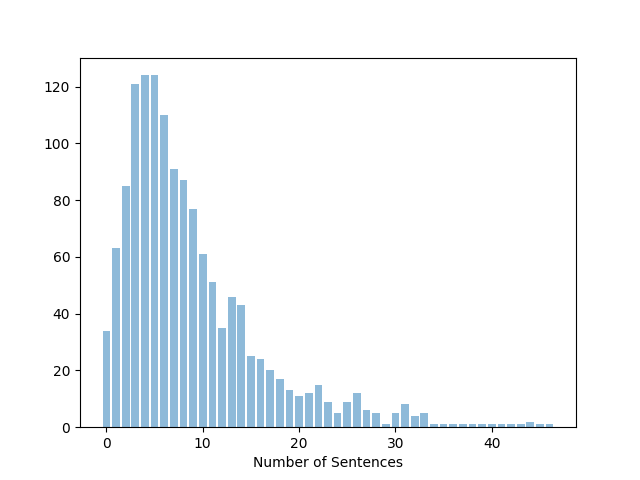
\includegraphics[width=\linewidth]{segmentation_2star.png}
  \caption{Sentence segmentation of reviews with 2 stars}
  \label{fig:seg_2star}
\end{figure}

\begin{figure}[ht]
  \centering
  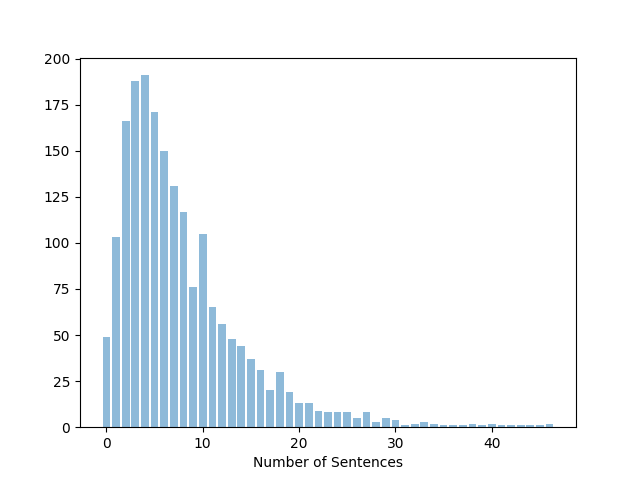
\includegraphics[width=\linewidth]{segmentation_3star.png}
  \caption{Sentence segmentation of reviews with 3 stars}
  \label{fig:seg_3star}
\end{figure}

\begin{figure}[ht]
  \centering
  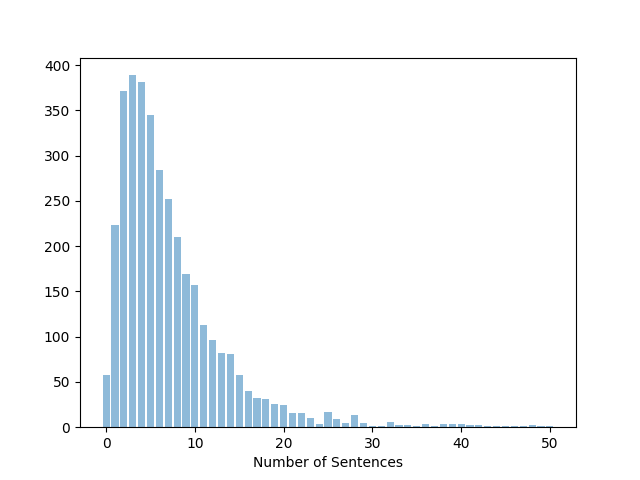
\includegraphics[width=\linewidth]{segmentation_4star.png}
  \caption{Sentence segmentation of reviews with 4 stars}
  \label{fig:seg_4star}
\end{figure}

\begin{figure}[ht]
  \centering
  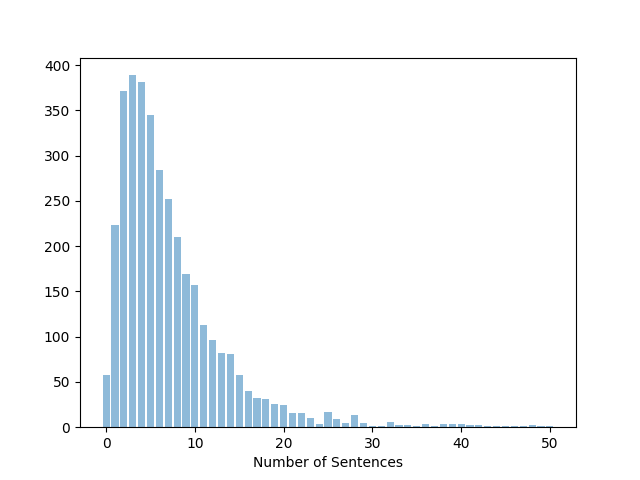
\includegraphics[width=\linewidth]{segmentation_4star.png}
  \caption{Sentence segmentation of reviews with 5 stars}
  \label{fig:seg_5star}
\end{figure}

\subsubsection{Discussions} Some observations in the distributions are notable and discussed. 

\begin{itemize}
\item Data distribution in all the 5 plots roughly follows the pattern of Right-Skewed Normal Distribution. Some sight differences are observed in the data distributions, which are statistically insignificant.
\item Most frequent length occurs at 5 sentences across the plots, which shows that regardless of the rating stars, people tend to write moderate length reviews. This indicates that reviews are generally short and simple piece of text with few cases being long and complex.
\item The data distributions skew farther towards right as the rating stars decrease. As shown the ranges of the x axis are \begin{math}[1,85]\end{math}, \begin{math}[1,74]\end{math}, \begin{math}[1,55]\end{math}, \begin{math}[1,71]\end{math}, \begin{math}[1,60]\end{math} from 1 to 5 stars. This gives the conclusion that there is higher possibility for the reviewers to write very long negative comments, and the neutral comments are usually shorter. It somehow reveals the interesting fact that people would like to comment more on the things that disappoint or irritate them rather than compliment more on the things that entertain them.
\item The data distributions reaches a higher number as a whole when the rating stars increases. As shown the ranges of y axis are \begin{math}[0,219]\end{math}, \begin{math}[0,124]\end{math}, \begin{math}[0,191]\end{math}, \begin{math}[0,389]\end{math}, \begin{math}[0,929]\end{math} and the total number of comments for each rating are: 2306, 1372, 1904, 3559, 6159, from 1 start to 5 stars. This reveals another interesting fact that more high-rating comments than low-rating ones, that is people are more likely to review something entertaining than something disappointing or even irritating.
\end{itemize}

\subsubsection{Verification} The sentence segmentation tool used is the Punkt Sentence Tokenizer from Python NLTK package. Sample code is given below.
\begin{verbatim}
from nltk import sent_tokenize
for r in reviews:
    r['sentences']=sent_tokenize(r['text'])
\end{verbatim}

5 reviews, including both short and long reviews, are randomly selected to verify whether the sentence segmentation tool detects the sentence boundaries correctly. 
\begin{itemize}
\item{Example 1 (1 sentences)}:["I love love their Kalbi, I always order it the sauce is what makes it really good..hmm think I wanna eat that today.i didn't like their noodles to sweet.."]
\item{Example 2 (4 sentences)}:["The food was amazing.", "The filet and lobster tail was perfect.", "Its hard to beat a great steak and lobster tail for under \$30.", "Also the service was on point."]
\item{Example 3 (7 sentences)}:["Visited for the first time today.", "Red door signature facial.", "Jordan was amazing.", "My skin looks and feels smoother and moisturized.", "The atmosphere is so elegant and relaxing .", "I'll be be back again soon!", "!"]
\item{Example 4 (13 sentences)}:["Worst customer service I have ever received.", "This is the first review on yelp I have left that is not 5 stars.", "I moved into a new house a promptly had an issue with the pool.", "I did not have a pool company so relied on my home warranty company First American and they send Aarons Pool.", "It was a disaster from start to finish.", "They had a no-show for my first scheduled appointment after waiting over a week.", "The second appointment he entered my backyard without my permission and supposedly replaced a capacitor.", "The company REFUSED to have someone go back to my house show me the repair!", "After being unable to resolve my complaints with the technician I called the office.", "The office refused to send the tech back out to prove to me the work had been done and HUNG UP ON ME.", "The capacitor did NOT fix my issue IF it was replaced.", "The warranty company First American sent out another company who diagnosed and replaced the pool pump all under warranty.", "Aaron's Pool was obviously only interested in making a quick dollar from the warranty company and not gaining a potential lifelong customer."]
\item{Example 5 (33 sentences)}: ["I went to Mayworth with a neighbor and I truly enjoyed myself.", "I remember visiting this establishment when it was Center Street Tavern ( probably said the name wrong) years ago.", "Nevertheless, I truly enjoyed Mayworth.", "From the time we walked in until the time we left,  Dana took care of us.", "Her hospitality was outstanding.", "The pub is very inviting and cozy.", "I really wanted to stay longer, but I had things to do.", "I order the Jamaican jerk wings entree with a side of sweet potato waffle fries.", "The Jamaican Jerk was not to my liking.", "I felt it wasn't spicy or seasoned at all.", "However, the fries were so delicious.", "Dana suggested mayo with it, and I said no thanks, but do you have something else?", "She had me to try the chipotle sauce and man was it good.", "Afterwards, Dana asked me about my wings.", "I had to be honest, I just told her I didn't like them at all.", "She immediately said she would get me another flavor wing if I wanted.", "I said yes, and requested the  hot wings.", "When the owner found out that I wasn't satisfied he immediately came over to our table to talk with me.", "Again, I told him about the wings.", "He assured me that he would take care of me.", "The wings came out and boy were they good!", "I really enjoyed them.", "The owner comes back over and asked if I was pleased with the wings and I said yes and thanked him for taking care of me.", "This owner went above and beyond what most owners would do.", "I never got a bill so I had to asked Dana for it.", "To my surprise there was no billed because the owner took care of it.", "Most customer would say thank you right off, but not me!", "I wanted to fuss with the waitress about the owner taking care of my bill!", "He didn't have to do it, but he did and for that courtesy I'm so grateful.", "He will have my business from now on.", "This is the kind of establishment you want to embark on.", "You know you're going to be cared for here.", "Thank you for the love shown."]
\end{itemize}

Example 1 gives a typical case where Punkt Sentence Tokenizer fails. While it should have segmented the text into multiple sentences, Punkt is mislead by the misuse of punctuation, ".." as the end of sentence, no space after "." and starting a sentence without capitalization, and Punkt considers the text as one single sentence. Example 3 gives another case where informal expression, in this case "!!" as the sentence boundary, confuses the tokenizer. Punkt consider "!!" to be two sentences rather than one unit of punctuation. Example 2, 4 and 5 are correctly segmented, mainly because these reviews, especially the longer two reviews, tends to have better grammar in favor of the tokenizer.

\subsection{Tokenization and Stemming}
The tokenization and stemming are performed on the restaurant reviews and the distributions of the number of tokens given by tokenization and stemming are shown in plots. In each plot, the x-axis is the length of a review in number of words and the y-axis is the number of reviews of such length. Figure \ref{fig:token_stem_separate} shows the distribution after tokenization and Figure \ref{fig:token_stem_combined} shows that after stemming.

\begin{figure}[ht]
  \centering
  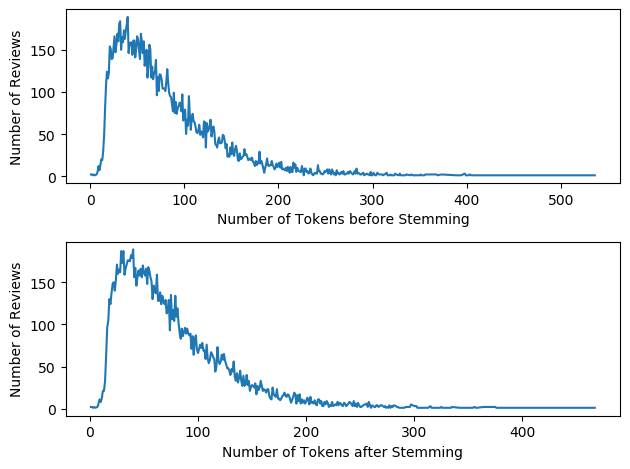
\includegraphics[width=\linewidth]{token_stem_separate.png}
  \caption{Tokenization and stemming result of reviews}
  \label{fig:token_stem_separate}
\end{figure}

\begin{figure}[ht]
  \centering
  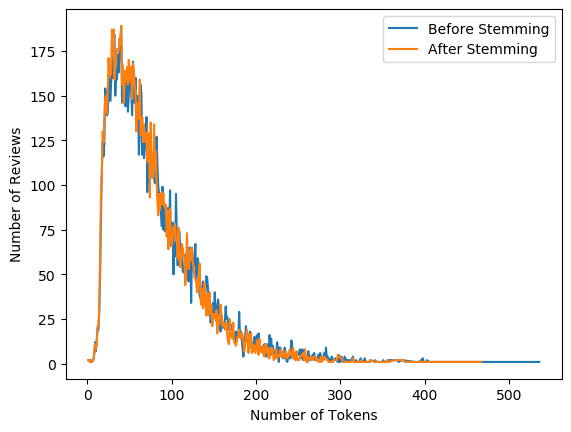
\includegraphics[width=\linewidth]{token_stem_combined.png}
  \caption{Combined tokenization and stemming result of reviews}
  \label{fig:token_stem_combined}
\end{figure}


The work tokenization tool used is the Treebank Word Tokenizer from Python NLTK package. Sample code is given below.
\begin{verbatim}
from nltk.tokenize import word_tokenize
...# vectorize word_tokenize function
for r in reviews
    r['words']=word_tokenize(r['text'])
\end{verbatim}

Port Stemmer is used to perform stemming on each token. Sample code is given below.
\begin{verbatim}
from nltk import PorterStemmer
stemmer=PorterStemmer()
...# vectorize stemmer.stem function
for r in reviews
    r['stems']=stemmer.stem(r['words'])
\end{verbatim}

\subsubsection{Discussion} Following are some discussions on the tokenization and stemming shown.
\begin{itemize}
\item After stemming is applied, the maximum number of tokens in a review changes from 536 to 467, while the minimum number of tokens remains to be 1.
\item Compared with the number of reviews of each length before stemming, the curve after stemming is generally more compact towards zero. Especially the number of tokens ranging from 50 to 80, the number of reviews of each length after stemming is larger than the one without stemming.
\end{itemize}

The top-20 most frequent words, excluding the stop words, before and after performing stemming are plotted in the histograms, \ref{fig:hist_token} and \ref{fig:hist_stem}. The stop words used in analysis are in the appendix of the report.

\begin{figure}[ht]
  \centering
  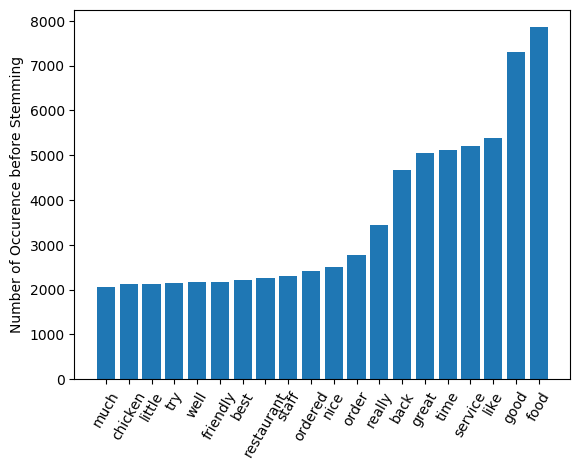
\includegraphics[width=\linewidth]{frequent_token.png}
  \caption{Histogram for top 20 frequent words before stemming}
  \label{fig:hist_token}
\end{figure}

\begin{figure}[ht]
  \centering
  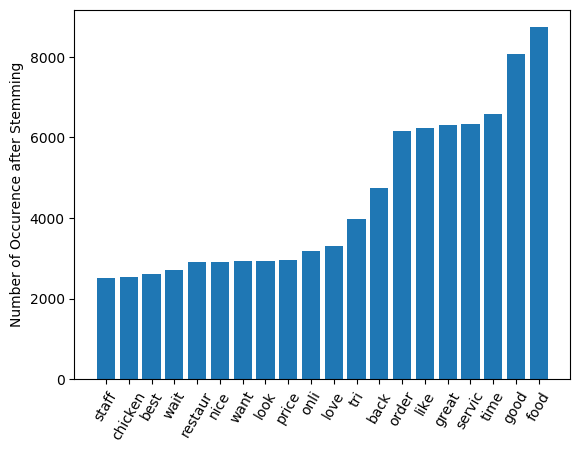
\includegraphics[width=\linewidth]{frequent_stem.png}
  \caption{Histogram for top 20 frequent words after stemming}
  \label{fig:hist_stem}
\end{figure}

\subsubsection{Discussion} The words expected and not expected to be popular given the nature of the restaurant reviews, and the effect of stemming on the top 20 list are discussed below.

\begin{itemize}
\item The words that are expected to be popular include: "food", "good", "like", "service", "great", "order", "staff", "friendly", "restaurant", "price". Those words are expected to be highly associated with the context of reviews on food and restaurant.
\item The words that are not expected to be so popular include: "time", "back", "look". Although those words are also commonly used in reviews, there are not expected to be so popular, ‘time’ and ‘back’ are even more popular than ‘restaurant’ both for with or without stemming, and ‘look’ is more popular than ‘restaurant’ after stemming is performed.
\item The stemming leads to an increase in the number of occurrences for most of the words since the words with the same stem but different affixes are also counted. Some of the words such as order, like, time even have an increase in rank.
\end{itemize}

\subsection{POS Tagging}
POS tagging are applied to 5 selected sentences from the data. Sample code is given below.
\begin{verbatim}
from nltk import pos_tag
reviews['pos']=reviews['words'].apply(pos_tag)
\end{verbatim}

\subsubsection{Result} The following are POS tagging results for the 5 selected sentences:
\begin{itemize}
\item{Sentence 1}:Some/\textbf{DT} great/\textbf{JJ} Hawaiian/\textbf{JJ} food/\textbf{NN} and/\textbf{CC} friendly/\textbf{JJ} staff/\textbf{NN} !/\textbf{.}
\item{Sentence 2}:service/\textbf{NN} was/\textbf{VBD} just/\textbf{RB}  as/\textbf{RB} good/\textbf{JJ} as/\textbf{IN} the/\textbf{DT} food/\textbf{NN} !/\textbf{.} !/\textbf{.} !/\textbf{.}
\item{Sentence 3}:I/\textbf{PRP} 'm/\textbf{VBP} sad/\textbf{JJ}  that/\textbf{IN} this/\textbf{DT} restaurant/\textbf{NN} is/\textbf{VBZ} closed/\textbf{VBN} .../\textbf{:}
\item{Sentence 4}:Clean/\textbf{NNP} ,/\textbf{,} spacious/\textbf{JJ} ,/\textbf{,} quite/\textbf{RB} ,/\textbf{,} and/\textbf{CC} nice/\textbf{JJ} breakfast/\textbf{NN}
\item{Sentence 5}:One/\textbf{CD} of/\textbf{IN} the/\textbf{DT} best/\textbf{JJS} sushi/\textbf{NN} places/\textbf{NNS} in/\textbf{IN} Mississauga/\textbf{NNP} ./\textbf{.}
\end{itemize}

From the results above, it can be concluded that the results produced by the POS tagger is already fairly accurate. For example, some special words like Mississauga is correctly tagged as NNP, and punctuation such as ‘!', ‘,’, '...' are tagged differently.

\subsection{Most Frequent Adjectives for Each Rating}
To analyse the most frequent adjectives and the most indicative adjectives with regards to the rating level of the reviews, the tagged tokens of each review from previous section are used to find their frequencies. The adjectives from the reviews of each rating are firstly extracted. The number of times a certain adjective appeared in the list of tokens is then counted and the respective percentage of the word is calculated. The most frequent adjectives is afterwards listed. Sample code is given below:

\begin{verbatim}
from nltk import FreqDist

for i in [1,2,3,4,5]:
    adj=[] 
    for r in reviews:
        if r['stars']==i:
            adj += [word for word,tag 
                    in r['pos_tag'] if tag=='JJ']
    adj_freqdist = FreqDist(adj)
\end{verbatim}

The formula to analyse the indicativeness of adjectives is as below.

Let \begin{math}P(w|Ri)\end{math} be the probability of observing word \begin{math}w\end{math} in all reviews with rating star \begin{math}i\end{math}, and let \begin{math}P(w)\end{math} be the probability of observing word \begin{math}i\end{math} in all reviews, then relative entropy for word w can be computed as: \begin{equation}
    P(w|R1)\times log(\frac{P(w|R1)}{P(w)})
\end{equation}

Following the formula, in addition to measuring the frequencies in respect to each rating, the frequencies of each adjective in the context of the entire data are also measured.

\subsubsection{Result} The result of this section is given in Table \ref{tab:adj1} and \ref{tab:adj2}:

\begin{table}
  \caption{Adjectives and their frequency}
  \label{tab:adj1}
  \begin{tabular}{lllll}
    \toprule
    Star & Word & Frequency \\
    \midrule
    1 & good & 633 \\
    & other & 532 \\
    & bad & 433 \\
    & new & 319 \\
    & first & 313 \\
    2 & good & 742 \\
    & other & 381 \\
    & great & 284 \\ 
    & bad & 236 \\
    & nice & 209 \\
    3 & good & 1453\\
    & other & 531 \\
    & great & 474 \\ 
    & nice & 419 \\ 
    & little & 375 \\
    4 & good & 2494 \\
    & great & 1480 \\ 
    & nice & 775 \\
    & other & 740 \\
    & little & 684 \\
    5 & great & 2586\\
    & good & 1944\\
    & friendly & 910\\
    & delicious & 887\\
    & nice & 832 \\
\end{tabular}
\end{table}

\begin{table}
  \caption{Adjectives and their indicativeness}
  \label{tab:adj2}
  \begin{tabular}{lllll}
    \toprule
    Star & Word & Frequency \\
    \midrule
    1 & other & 0.1054\\ 
    & bad & 0.1021\\ 
    & good & 0.0930\\ 
    & new & 0.0681\\ 
    & last & 0.0645\\
    2 & good & 0.1801\\ 
    & other & 0.1011\\ 
    & bad & 0.0685\\ 
    & great & 0.0530\\ 
    & same & 0.0500\\
    3 & good & 0.2847\\ 
    & other & 0.1004\\ 
    & nice & 0.0771\\ 
    & little & 0.0704\\ 
    & great & 0.0688\\
    4 & good & 0.2760\\ 
    & great & 0.1550\\ 
    & nice & 0.0828\\ 
    & little & 0.0741\\ 
    & other & 0.0731\\
    5 & great & 0.2345\\ 
    & good & 0.1383\\ 
    & delicious & 0.0804\\
    & friendly & 0.0771\\ 
    & nice & 0.0647\\
\end{tabular}
\end{table}


\section{Noun-Adjective Pair Summarizer}
Noun-Adjective pairs are extracted from reviews of 5 randomly selected business, 100 reviews each. Each pair has a count to denote the frequency. Five most frequent Noun-Adjective pairs for each business are selected to discuss the correctness of this summarizer corresponding to the reviews text. 

\subsection{Example 1: Baro}
\begin{table}
  \caption{Example 1 Baro}
  \label{tab:n_adj_1}
  \begin{tabular}{lllll}
    \toprule
    Noun-Adjective pair & Frequency \\
    \midrule
    ('food', 'good') & 12\\
    ('food', 'great') & 11\\
    ('floor', 'second') & 8\\
    ('floor', '2nd') & 7\\
    ('food', 'amazing') & 6\\
\end{tabular}
\end{table}

By observing the Noun-Adjective pairs shown in Table \ref{tab:n_adj_1}, this business can be summarized to be a restaurant with delicious food. Among the 5 most frequently appeared pairs, (food, good) (food, great) (food, amazing) take up 3 positions. 
After reading some of the reviews, we find that most customers do enjoy the food hepre and this matches the result generated by the summarizer.

\subsection{Example 2: Sierra Gold}
\begin{table}
  \caption{Example 2 Sierra Gold}
  \label{tab:n_adj_2}
  \begin{tabular}{lllll}
    \toprule
    Noun-Adjective pair & Frequency \\
    \midrule
    ('hour', 'happy') & 21\\
    ('food', 'good') & 17\\
    ('time', 'first') & 11\\
    ('staff', 'friendly') & 9\\
    ('service', 'good') & 7\\
\end{tabular}
\end{table}

The business is a bar, such that the pair: (hour, happy) has a very high frequency in the reviews, as shown in Table \ref{tab:n_adj_2}. Although the top 5 frequent pairs are positive, a number of the reviews are actually negative. However, negative reviews are mostly describing some complex situations which cannot be extracted to noun-adjective pairs.

\subsection{Example 3: Octagon}
\begin{table}
  \caption{Example 3 Octagon}
  \label{tab:n_adj_3}
  \begin{tabular}{lllll}
    \toprule
    Noun-Adjective pair & Frequency \\
    \midrule
    ('school', 'old') & 30\\
    ('bread', 'garlic') & 19\\
    ('medium', 'rare') & 15\\
    ('food', 'good') & 12\\
    ('glass', 'stained') & 11\\
\end{tabular}
\end{table}

This business is a very well-known steak house existed for a long time. As shown in Table \ref{tab:n_adj_3} (school, old) is the most frequently appeared Noun-Adjective pair. Many customers’ review mentioned that they have hard this long time ago and came because its famous reputation. Although upon seeing this pair, we can understand what it wants to express, a problem is old-school can actually be written as one word (Adjective) that describes a style. 

Also, (medium, rare) appeared many times since this business is a steak house, medium-rare is somehow combined with the order of steak. But the same problem as ‘old school’ is medium-rare is actually one word (Adjective) that describes how a steak will be cooked.

However, from observations of the summarizer, we can see that (food, good) has lower rank compared with others. And it is true that after seeing some of the reviews we found that food here does not reach many customers’ expectations.

In this way, we say that this summarizer overall correctly generalizes the key characteristic of this business. But the Noun-Adjective form Adjective word cannot be actually correctly identified.

\subsection{Example 4: Novanta}
\begin{table}
  \caption{Example 4 Novanta}
  \label{tab:n_adj_4}
  \begin{tabular}{lllll}
    \toprule
    Noun-Adjective pair & Frequency \\
    \midrule
    ('pizza', 'good') & 18\\
    ('pizza', 'amazing') & 9\\
    ('staff', 'friendly') & 8\\
    ('service', 'great') & 7\\
    ('food', 'great') & 7\\
\end{tabular}
\end{table}

This is a Pizza restaurant, the Noun-Adjective pairs reflect about the business.

\subsection{Example 5: Chico's}
\begin{table}
  \caption{Example 5 Chico's}
  \label{tab:n_adj_5}
  \begin{tabular}{lllll}
    \toprule
    Noun-Adjective pair & Frequency \\
    \midrule
    ('salsa', 'good') & 12\\
    ('food', 'Mexican') & 11\\
    ('food', 'good') & 10\\
    ('salsa', 'great') & 7\\
    ('food', 'fast') & 6\\
\end{tabular}
\end{table}
The business is a Mexican food restaurant. The comments do mention a lot about the good salsa in this restaurant. And the food is fast and good. the Noun-Adjective summarizer correctly generates keywords of the business.

\section{Application}
This application aims to understand how reviewers like the restaurant by sentiment analysis over text. We begin with some pretrained sentiment analysis tools provided in various libraries.  

\subsection{NLTK Vader Sentiment Analysis}

Vader tool\cite{Vader} uses the Bag of Words approach, a dictionary of words assigned with sentiment value from -1 to 1 for degree of positive and negative, and a heuristics function for depending adverb phrase. 

For example, the negative adjective “dumb” gives the sentiment of -0.55, and the pharse “so dumb” adds the intensity and gives an overall -0.72. 

Another example, although the positive verb “like” raise the sentiment to 0.36, heuristics function flips the sentiment of “do not like” because “like” in this case follows a negation. Vader’s heuristics function takes care of some subtle details in the sentence, such as the negation here.

One disadvantage of this approach is that it could not estimate the intensity for unseen word and classify it as neutral by default.

\subsection{Flair Sentiment Analysis}

Flair’s sentiment classifier, developed by Zalando Research group\cite{Flair}, is based on a character-level Long Short-Term Memory (LSTM)\cite{LSTM} neural network.

LSTM neural network has the feedback connections and can not only process single data point but also the entire sequences of data. Flair takes sequences of letters and words into account when evaluating the overall sentiment of the sentences.

Similar to Vader, negations and adverb phrase as intensifier are handled. An advantage of Flair is that it can predict a sentiment for unseen words, such as misspelt words.

\subsection{Stanford NLP Parser}

Stanford NLP Parser applies the POS tagging to the input sentence and returns the dependency tree and typed dependencies tree. POS tagging focuses on the detailed relationships between words and phrases with high accuracy.

Stanford NLP Parser has advantage over detecting negation expressions, such as “bad”, “really bad”, and“not good”, with typed dependencies. However, Some sophisticated process would be required to generalize word-level POS tagging dependencies to sentence-level or text-level sentiment. 

\subsection{Application Development}
The application is further developed  based on the two libraries evaluated, NLTK Vader and Flair. 

First, sentiment analysis over the entire text, that is model evaluates the sentence-level relationship and then gives overall text sentiment, is experimented. It performs well over the text at the expense of long execution time, 2.54s for a 301-word which makes it unscalable to the large dataset.

Sentence-level sentiment analysis is in fact not necessary, because of the nature of the review text. It is commonly observed that review is composed of straightforward and logic-independent sentences. Besides, reviewers tend to spend more effort on things they care about most, i.e. write several long sentences to describe.

This motivates us to the weighted-sentiment value. Review test is first segmented into sentences and record the word count for each sentence. Sentiment analysis tools, Vedar and Flair, give the sentiment values of the sentences. Sentiment value for overall text is then calculated from the sentiment values of the sentences weighted average by word counts.

To examine the accuracy of two models and our weighted-analysis approach, we compare our labels to the star rated by the reviewer. Two review texts below are examples where Vader and Flair mislabel the positive and negative.

Examples over 20 review samples are recorded in the spreadsheet in the output directory of the source code.

\subsection{Example 1 Failure of Flair}
\subsubsection{Review Text}“Love this place downtown but the Scottsdale location has no manners. Sat at bar for 10 min while bartender ignored us. No menu, no water. We walked out and they could have cared less.”

Sentiment analysis result are shown in Table \ref{tab:eg1}
\begin{table}
  \caption{Sentiment Analysis of Example 1}
  \label{tab:eg1}
  \begin{tabular}{lllll}
    \toprule
    Sentence & Star & Vader & Flair \\
    \midrule
    1 & & -0.0516 & 0.9997\\
    2 & & -0.3182 & 0.9987\\
    3 & & -0.5267 & 0.9868\\
    4 & & 0.4215 & 0.9962\\
    \bottomrule
    Overall & 1 & -0.0607 & 0.9970\\
\end{tabular}
\end{table}

\subsection{Example 2 Failure of Vader}

"I have no idea what the owner's problem is, but he's incredibly rude. His wife, on the other hand is super nice (an odd mix). Great space, rude owner and the coffee is average."

Sentiment analysis result are shown in Table \ref{tab:eg2}
\begin{table}
  \caption{Sentiment Analysis of Example 1}
  \label{tab:eg2}
  \begin{tabular}{lllll}
    \toprule
    Sentence & Star & Vader & Flair \\
    \midrule
    1 & & -0.7839 & -0.9944\\
    2 & & 0.8225 & -0.9265\\
    3 & & -0.4732 & 0.9997\\
    \bottomrule
    Overall & 1 & 0.0158 & -0.4732\\
\end{tabular}
\end{table}

\subsection{Discussion} Possible explanation for failure observed above are:
\begin{itemize}
\item The possible reason could be the reviewer’s definition for the level of satisfaction represented by each star given by themselves is different. For example, customer A and customer B both write the same sentence, “Great food but rude service”, in the review, however the star given by A is 2 while B is 1. It occurs could just because B is more cared about the service provided while A may focus more on the food.
\item Weighted average is calculated in a way such the weight for each sentence is calculated based on their length in terms of words. Some keyword may not be sufficiently highlighted in this case.
\item The fact the model’s training data set is from IMDB’s dataset, a movie review website’s dataset, which might not perfectly reflect the conditions of restaurant reviews.
\end{itemize}

\begin{acks}
To Dr. Aixin Sun, for teaching Natural Language Processing Course.
\end{acks}

\bibliographystyle{ACM-Reference-Format}
\bibliography{ntu-191011-base}

\appendix
\section{Stopwords}
\subsection{Stop words provided by NLTK}
i, me, my, myself, we, our, ours, ourselves, you, you're, you've, you'll, you'd, your, yours, yourself, yourselves, he, him, his, himself, she, she's, her, hers, herself, it, it's, its, itself, they, them, their, theirs, themselves, what, which, who, whom, this, that, that'll, these, those, am, is, are, was, were, be, been, being, have, has, had, having, do, does, did, doing, a, an, the, and, but, if, or, because, as, until, while, of, at, by, for, with, about, against, between, into, through, during, before, after, above, below, to, from, up, down, in, out, on, off, over, under, again, further, then, once, here, there, when, where, why, how, all, any, both, each, few, more, most, other, some, such, no, nor, not, only, own, same, so, than, too, very, s, t, can, will, just, don, don't, should, should've, now, d, ll, m, o, re, ve, y, ain, aren, aren't, couldn, couldn't, didn, didn't, doesn, doesn't, hadn, hadn't, hasn, hasn't, haven, haven't, isn, isn't, ma, mightn, mightn't, mustn, mustn't, needn, needn't, shan, shan't, shouldn, shouldn't, wasn, wasn't, weren, weren't, won, won't, wouldn, wouldn't, 

\subsection{Additional stop words utilized}
The, n't, I, 's, We, get, would, It, one, place, They, go, This, 've, got, us, my, could, also, even, 'm, always, came, come, still, made, said, going, know, If, day, 're, two, 2, say, take, way, ever, give, told, eat, minutes, around, So, asked, see, There, since, 'll, took, She, He, You, next, But, 3, And, 5, When, every, A, something, tried, ca, Not, everything, 'd, called, done, coming, things, wa, thi, veri, realli, becaus, alway, ha, ani, use, reallyThis, My, make, went, ask, definit, definitely, work, thing

\end{document}
\endinput
